\setcounter{framenumber}{304}
\begin{frame}
  \LectureNo{10}
  \maketitle
\end{frame}

\begin{frame}{Overview}
\tableofcontents
\end{frame}

\section{Rehash}
\begin{frame}{Rehash}
	
\begin{itemize}
	
		\item \alert{A model interprets the signature by assigning denotation to every constant, a function to every function symbol, and an $n$-ary relation to every $n$-ary relation symbol.}
		
		\item An assignment in a model tells us what the variables denote. It plays the role of the context in natural language. 
	
		\item We can recursively calculate the denotation of arbitrary terms in a model under an assignment.
		
		\item We can recursively calculate the truth-value of a formula relative to a model under an assignment.
		
		\item Validity is defined as in every logic as truth-preservation across models.
		
		\item \alert{The Deduction Theorem holds for first-order logic but doesn't lead to decidability.}
										
	\end{itemize}

\end{frame}

\begin{frame}


	
	\begin{center}
		\begin{tabular}{c}
		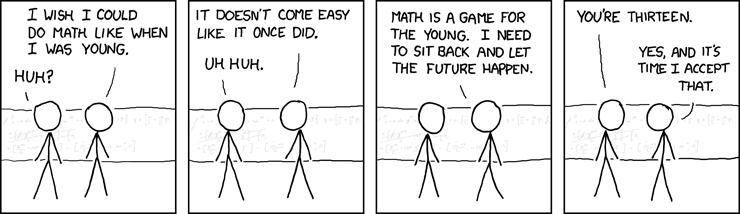
\includegraphics[width=60ex]{xkcd-tofts}\\[-1ex]
		{\tiny \textcopyright~\url{https://xkcd.com/447/}, CC BY-NC 2.5}
		\end{tabular}
		\end{center}

\end{frame}
		

\section{10. Tableaux for First-Order Logic}
\subsection{10.1 Overview}

\begin{frame}{10.1 Overview}

	\begin{itemize}
		
		\item (10.1.1) Things work \emph{very} similar to how they work in propositional logic:
		\[\Gamma\vDash\phi\text{ iff }\Gamma\cup\{\neg\phi\}\text{ is unsatisfiable}\]

		\item (10.1.2) However, things don't work quite as \emph{algorithmically} as before:
		\begin{itemize}
			
			\item We might get \emph{infinite} tableaux.
		
		\end{itemize}

		\item (10.1.3) First-order logic is undecidable: 
				
		\begin{itemize}
		
			\item \textbf{Theorem}(Church and Turing 1935/36)\textbf{.} There exists no effective algorithm that for every inference after finitely many steps correctly determines whether the premises entail the conclusion in first-order logic.
			
		\end{itemize}
		
		\item (10.1.4) We proceed in steps:
		
			\begin{itemize}
			
				\item \S10.2 Simple Tableaux
				
				\item \S10.3 Tableaux with Identity
				
				\item \S10.4 Tableaux with Functions
			
			\end{itemize}

	\end{itemize}

\end{frame}

\subsection{10.2 Simple Tableaux}

\begin{frame}{Reminder}

		
			\begin{center}		
					\begin{prooftree}
					{
					line numbering=false,
					line no sep= 2cm,
					for tree={s sep'=5mm},
					single branches=true,
					close with=\xmark
					}
					[\neg\neg \phi [\phi ] ]
					\end{prooftree}
					%
					\begin{prooftree}
					{
					line numbering=false,
					line no sep= 2cm,
					for tree={s sep'=5mm},
					single branches=true,
					close with=\xmark
					}
					[\phi\land\psi [\phi [\psi ] ] ]
					\end{prooftree}
					%
					\begin{prooftree}
					{
					line numbering=false,
					line no sep= 2cm,
					for tree={s sep'=5mm},
					single branches=true,
					close with=\xmark
					}
					[\neg (\phi\land\psi) [\neg \phi ] [\neg \psi ] ]
					\end{prooftree}
					%
					\begin{prooftree}
					{
					line numbering=false,
					line no sep= 2cm,
					for tree={s sep'=5mm},
					single branches=true,
					close with=\xmark
					}
					[\phi\lor\psi [\phi ] [\psi ] ]
					\end{prooftree}
					%
					\begin{prooftree}
					{
					line numbering=false,
					line no sep= 2cm,
					for tree={s sep'=5mm},
					single branches=true,
					close with=\xmark
					}
					[\neg(\phi\lor\psi) [\neg\phi [\neg\psi ] ] ]
					\end{prooftree}

					\vspace{2ex}

					\begin{prooftree}
					{
					line numbering=false,
					line no sep= 2cm,
					for tree={s sep'=5mm},
					single branches=true,
					close with=\xmark
					}
					[\neg (\phi\to\psi) [\phi [\neg \psi ] ] ]
					\end{prooftree}
					%
					\begin{prooftree}
					{
					line numbering=false,
					line no sep= 2cm,
					for tree={s sep'=5mm},
					single branches=true,
					close with=\xmark
					}
					[\phi\to\psi [\neg \phi ] [\psi ] ]
					\end{prooftree}
					%
					\begin{prooftree}
					{
					line numbering=false,
					line no sep= 2cm,
					for tree={s sep'=5mm},
					single branches=true,
					close with=\xmark
					}
					[\phi\leftrightarrow \psi [\phi [\psi] ] [\neg \phi [\neg \psi] ] ]]
					\end{prooftree}
					%
					\begin{prooftree}
					{
					line numbering=false,
					line no sep= 2cm,
					for tree={s sep'=5mm},
					single branches=true,
					close with=\xmark
					}
					[\neg(\phi\leftrightarrow \psi) [\phi [\neg \psi] ] [\neg \phi [ \psi] ] ]]
					\end{prooftree}

				\end{center}
				
				

\end{frame}

\begin{frame}{(10.2.2) Parameters}

	\begin{itemize}
		
		\item We need to talk about arbitrary objects. For this purpose, we introduce \emph{parameters}:
		
		\[\mathsf{Par}=\{p,q,r,p_1, p_2, \mathellipsis\}\]
		
		\item Don't confuse them with sentence letters!
		
		\item They work just like constants: \[\forall x(P(x)\to \exists y(R(x,y)\land R(y,p))\]
		
		\item They also get interpreted like constants: \[p^\mathcal{M}\in D^\mathcal{M}\]
		
		\item Nothing to see in the truth-conditions either:
		
		\[\mathcal{M},\alpha\vDash P(p)\text{ iff }p^\mathcal{M}\in P^\mathcal{M}\]
	
	\end{itemize}


\end{frame}

\begin{frame}{(10.2.4) Quantifier Rules}

		\begin{center}
\begin{prooftree}
{
line numbering=false,
line no sep= 2cm,
for tree={s sep'=10mm},
single branches=true,
close with=\xmark
}
[\neg \forall x\varphi
	[\exists x\neg\varphi ]
]
\end{prooftree}\hspace{4ex}
\begin{prooftree}
{
line numbering=false,
line no sep= 2cm,
for tree={s sep'=10mm},
single branches=true,
close with=\xmark
}
[\neg \exists x\varphi
	[\forall x\neg \varphi ]
]
\end{prooftree}
\\[4ex]

\begin{prooftree}
{
centered,
line numbering=false,
line no sep= 2cm,
for tree={s sep'=10mm},
single branches=true,
close with=\xmark
}
[\exists x\varphi
	[{(\varphi)[x:=p]^\dagger} ]
]\end{prooftree}\hspace{4ex}
\begin{prooftree}
{
line numbering=false,
line no sep= 2cm,
for tree={s sep'=10mm},
single branches=true,
close with=\xmark
}
[\forall x\varphi
	[{(\varphi)[x:=a]^\ddagger} ]
]
\end{prooftree}
\end{center}

\vspace{2ex}

$\dagger$: where $p\in\mathsf{Par}$ is any parameter not on the branch already.

$\ddagger$: where $a\in\mathcal{C}\cup\mathsf{Par}$ is any \emph{constant or parameter} already on the branch, or an arbitrary ``fresh'' parameter if there are none.


\end{frame}

\begin{frame}{(10.2.5) The $\exists$ Rule}

	\begin{itemize}
	
		\item You need a fresh parameter \emph{every time}:
		
		\begin{center}
\begin{prooftree}
{
centered,
line numbering=false,
line no sep= 2cm,
for tree={s sep'=10mm},
single branches=true,
close with=\xmark
}
[{\exists x\exists yR(x,y)}
	[{\exists yR(p,y)}
		[{R(p,q)}
		]
	]
]\end{prooftree}
\end{center}
	
		\item Idea: If $\exists x\phi$ is true, all we know is that some object satisfies $\phi$. Since we don't know which one, we pick a new parameter.
	
	\end{itemize}	

\end{frame}
\begin{frame}{(10.2.6) The $\forall$ Rule}

	\begin{itemize}
	
		\item The rule needs to be applied to \emph{every} term on the branch: 
		
			\begin{center}{\scriptsize
\begin{prooftree}
{
centered,
line numbering=false,
line no sep= 2cm,
for tree={s sep'=10mm},
single branches=true,
close with=\xmark
}
[{\forall xP(x)}, grouped
	[Q(a), grouped
		[{R(q,b)}, grouped
			[P(a)
				[{P(q)}
					[P(b)]
				]
			]
		]
	]
]\end{prooftree}}
\end{center}

	\item Even if they pop up later:
	
		\begin{center}{\scriptsize
\begin{prooftree}
{
centered,
line numbering=false,
line no sep= 2cm,
for tree={s sep'=10mm},
single branches=true,
close with=\xmark
}
[{\forall xP(x)}, grouped
	[{\exists yR(a,y)}, grouped
		[{P(a)}
			[{R(a,p)}
				[P(p)]
			]
		]
	]
]\end{prooftree}}
\end{center}
	
	\end{itemize}


\end{frame}

\begin{frame}{(10.2.7) Fresh Parameters}


	\begin{itemize}
	
		\item Idea: Each term on the branch denotes something, so if $\forall x\phi$ is true, then also that thing is $\phi$.
		
		\item If there are no constants or parameters around, we need to introduce them:
		
		\begin{center}	
\begin{prooftree}
{
centered,
line numbering=false,
line no sep= 2cm,
for tree={s sep'=10mm},
single branches=true,
close with=\xmark
}
[{\forall xP(x)}, grouped
	[{\forall x(P(x)\to Q(x))}, grouped
		[{P(p)}
			[{P(p)\to Q(p)}
				[\neg P(p)]
				[Q(p)]
			]
		]
	]
]\end{prooftree}
\end{center}

		\item This is because domains are non-empty.
	
	
	\end{itemize}


\end{frame}

\begin{frame}{(10.2.9) Remaining Definitions}


	\begin{itemize}
	
		\item A branch $B$ is closed iff there is some $R(t_1, \mathellipsis, t_n),\neg R(t_1, \mathellipsis, t_n)\in B$; otherwise $B$ is open.
		
		\item A tableau is closed iff every branch is closed; otherwise it's open.
		
		\item $\Gamma\vdash\phi$ iff the complete tableau for $\Gamma\cup\{\neg\phi\}$ is closed.
	
	\end{itemize}

\end{frame}

\begin{frame}{(10.2.10.i) Example}

\begin{center}

\begin{prooftree}
{
proof statement format={centered},
to prove={\forall xP(x)\vdash \exists xP(x)},
line numbering=false,
for tree={s sep'=10mm},
single branches=true,
close with=\xmark
}
[\forall xP(x), grouped 
	[\neg\exists xP(x), grouped
		[\forall x\neg P(x)
			[\neg P(p)
				[P(p), close
				]
			]
		]
	]
]
\end{prooftree}

\end{center}


\end{frame}


\begin{frame}{(10.2.10.ii) Example}

	\begin{center}
		{\small		\begin{prooftree}
{
proof statement format={centered},
to prove={\exists x(P(x)\land Q(x))\vdash \exists xP(x)\land \exists xQ(x)},
line numbering=false,
for tree={s sep'=10mm},
single branches=true,
close with=\xmark
}
[\exists x(P(x)\land Q(x)), grouped 
	[\neg(\exists xP(x)\land \exists xQ(x)), grouped
		[P(p)\land Q(p)
			[P(p)
				[Q(p)
					[\neg\exists xP(x)
						[\forall x \neg P(x)
							[\neg P(p), close]	
						]
					]
					[\neg\exists xQ(x)
						[\forall x \neg Q(x)
							[\neg Q(p), close]
						]
					]
				]
			]
		]
	]
]
\end{prooftree}}
	\end{center}


\end{frame}


\begin{frame}{(10.2.10.iv) Example}

\begin{center}{\small
			\begin{prooftree}
{
proof statement format={centered},
to prove={\forall xP(x)\lor\forall xQ(x)\vdash \forall x(P(x)\lor Q(x))},
line numbering=false,
for tree={s sep'=10mm},
single branches=true,
close with=\xmark
}
[\forall xP(x)\lor\forall xQ(x), grouped 
	[\neg\forall x(P(x)\lor Q(x)), grouped
		[\exists x\neg (P(x)\lor Q(x))
			[\neg (P(p)\lor Q(p))
				[\neg P(p)
					[\neg Q(p)
						[\forall xP(x)
							[P(p), close
							]
						]
						[\forall xQ(x)
							[Q(p), close
							]
						]
					]
				]
			]
		]
	]
]
\end{prooftree}}

\end{center}

\end{frame}


\begin{frame}{(10.2.10.v) Example}


\begin{center}
{\small
 \begin{prooftree}
{
proof statement format={centered},
to prove={\exists x\forall yR(x,y)\vdash \forall y\exists xR(x,y)},
line numbering=false,
for tree={s sep'=10mm},
single branches=true,
close with=\xmark
}
[{\exists x\forall yR(x,y)}, grouped 
	[{\neg\forall y\exists xR(x,y)}, grouped
		[{\forall yR(p_1,y)}
			[{\exists y\neg\exists xR(x,y)}
				[{\neg\exists xR(x,p_2)}
					[{\forall x\neg R(x,p_2)}
						[{R(p_1,p_2)}
							[{\neg R(p_1,p_2)}, close
							]
						]
					]
				]
			]
		]
	]
]
\end{prooftree}}

\end{center}

\end{frame}

\begin{frame}{(10.2.10.vii) Example}

\begin{center}{\scriptsize

 \begin{prooftree}
{
proof statement format={centered},
to prove={\vdash\neg \exists x(K(x)\land \forall y(\neg S(y,y)\leftrightarrow S(x,y)))},
line numbering=false,
for tree={s sep'=10mm},
single branches=true,
close with=\xmark
}
[{\neg \neg \exists x(K(x)\land \forall y(\neg S(y,y)\leftrightarrow S(x,y)))}
	[{\exists x(K(x)\land \forall y(\neg S(y,y)\leftrightarrow S(x,y)))}
		[{\exists x(K(x)\land \forall y(\neg S(y,y)\leftrightarrow S(x,y)))}
					[{(K(p)\land \forall y(\neg S(y,y)\leftrightarrow S(p,y)))}
						[{K(p)}
							[{\forall y(\neg S(y,y)\leftrightarrow S(p,y)))}
								[{\neg S(p,p)\leftrightarrow S(p,p)}
									[{\neg S(p,p)}
										[{S(p,p)}, close ]
									]
									[{S(p,p)}
										[{\neg S(p,p)}, close ]
									]
								]
							]
						]				
					]
		]
	]
]
\end{prooftree}

}\end{center}

\end{frame}

\begin{frame}{(10.2.11) \emph{Un}derivaibility}

 $\Gamma\nvdash\phi$ iff the tableau for $\Gamma\cup\{\neg\phi\}$ contains an open branch.

\begin{center}{\tiny		
\begin{prooftree}
{
proof statement format={centered},
to prove={\forall x(P(x)\lor Q(x))\nvdash \forall xP(x)\lor \forall xQ(x)},
line numbering=false,
for tree={s sep'=10mm},
single branches=true,
close with=\xmark
}
[\forall x(P(x)\lor Q(x)), grouped 
	[\neg(\forall xP(x)\lor \forall xQ(x)), grouped
		[\neg \forall xP(x)
			[\neg\forall xQ(x)
				[\exists x\neg P(x)
					[\exists x\neg Q(x)
						[\neg P(p)
							[\neg Q(q)
								[P(p)\lor Q(p)
									[P(q)\lor Q(q)
										[P(p), close
										]
										[Q(p)
											[P(q)]
											[Q(q), close]
										]
									]
								]
							]
						]
					]
				]
			]
		]
	]
]
\end{prooftree}}
\end{center}

\end{frame}

\begin{frame}{(10.2.12) Associated Models}

	\begin{itemize}
	
		\item For $B$ an open branch of a complete tableau, we define $\mathcal{M}_B$ by:
		\begin{enumerate}[(i)]
		
			\item $D^{\mathcal{M}_B}=\{a\in \mathcal{C}\cup Par: a\text{ occurs on }B\}$
			
			\item $a^{\mathcal{M}_B}=a$ for all $a\in \mathcal{C}\cup Par$
			
			\item $R^{\mathcal{M}_B}=\{(a_1, \mathellipsis, a_n): R(a_1, \mathellipsis, a_n)\in B\}$
		
		\end{enumerate}
	
		\item This is a \emph{term model}, the objects in the domain are terms.
	
	\end{itemize}

\end{frame}

\begin{frame}{(10.2.13.i) Example}

\begin{tabular}{c c}
\begin{minipage}{.5\linewidth}{\tiny
\begin{prooftree}
{
proof statement format={centered},
to prove={\forall x(P(x)\lor Q(x))\nvdash \forall xP(x)\lor \forall xQ(x)},
line numbering=false,
for tree={s sep'=10mm},
single branches=true,
close with=\xmark
}
[\forall x(P(x)\lor Q(x)), grouped 
	[\neg(\forall xP(x)\lor \forall xQ(x)), grouped
		[\neg \forall xP(x)
			[\neg\forall xQ(x)
				[\exists x\neg P(x)
					[\exists x\neg Q(x)
						[\neg P(p)
							[\neg Q(q)
								[P(p)\lor Q(p)
									[P(q)\lor Q(q)
										[P(p), close
										]
										[Q(p)
											[P(q)]
											[Q(q), close]
										]
									]
								]
							]
						]
					]
				]
			]
		]
	]
]
\end{prooftree}}
\end{minipage}&
\begin{minipage}{.5\linewidth}
\begin{itemize}
	\item[] $D^{\mathcal{M}_B}=\{p,q\}$
	\item[] $p^{\mathcal{M}_B}=p$
	\item[] $q^{\mathcal{M}_B}=q$
	\item[] $P^{\mathcal{M}_B}=\{q\}$
 	\item[] $Q^{\mathcal{M}_B}=\{p\}$
\end{itemize}
\end{minipage}
\end{tabular}

\end{frame}

\begin{frame}{(10.2.13.ii) Example}

\begin{tabular}{c c}
\begin{minipage}{.5\linewidth}{\tiny
	\begin{prooftree}
{
proof statement format={centered},
to prove={\forall x\forall y(R(x,y)\to R(y,x))\nvdash \forall xR(x,x)},
line numbering=false,
for tree={s sep'=10mm},
single branches=true,
close with=\xmark
}
[{\forall x\forall y(R(x,y)\to R(y,x))}, grouped
	[{\neg \forall xR(x,x)}, grouped
		[{\exists x\neg R(x,x)}
			[{\neg R(p,p)}
				[{\forall y(R(p,y)\to R(y,p))}
					[{R(p,p)\to R(p,p)}
						[{\neg R(p,p)} ]
						[{R(p,p)}, close ]
					]
				]
			]
		]
	]
]
\end{prooftree}}
\end{minipage}&
\begin{minipage}{.5\linewidth}
\begin{itemize}
	\item[] $D^{\mathcal{M}_B}=\{p\}$
	\item[] $p^{\mathcal{M}_B}=p$
	\item[] $R^{\mathcal{M}_B}=\emptyset$
\end{itemize}
\end{minipage}
\end{tabular}
\end{frame}

\begin{frame}{(10.2.13.iii) Example}

\begin{tabular}{c c}
\begin{minipage}{.5\linewidth}{\tiny
	\begin{prooftree}
{
proof statement format={centered},
to prove={\exists x (P(c)\to P(x))\nvdash \neg (P(c)\to \forall xP(x))},
line numbering=false,
for tree={s sep'=10mm},
single branches=true,
close with=\xmark
}
[{\exists x (P(c)\to P(x))}, grouped
	[{\neg (P(c)\to \forall xP(x))}, grouped
		[P(c)
			[\neg \forall xP(x)
				[\exists x\neg P(x)
					[\neg P(p)
						[P(c)\to P(p)
						[\neg P(c), close]
						[P(p)]
						]
					]
				]
			]
		]
	]
]
\end{prooftree}}
\end{minipage}&
\begin{minipage}{.5\linewidth}
\begin{itemize}
	\item[] $D^{\mathcal{M}_B}=\{c,p\}$
	\item[] $p^{\mathcal{M}_B}=p$
	\item[] $c^{\mathcal{M}_B}=c$
	\item[] $P^{\mathcal{M}_B}=\{c\}$
\end{itemize}
\end{minipage}
\end{tabular}
\end{frame}
\begin{frame}{(10.2.13.iv) Example}

\begin{tabular}{c c}
\begin{minipage}{.5\linewidth}{\tiny
			\begin{prooftree}
{
proof statement format={centered},
to prove={\nvdash \forall x\forall y(R(x,y)\to R(y,x))},
line numbering=false,
for tree={s sep'=10mm},
single branches=true,
close with=\xmark
}
[{\neg\forall x\forall y(R(x,y)\to R(y,x))}
	[{\exists x\neg\forall y(R(x,y)\to R(y,x))}
		[{\neg\forall y(R(p,y)\to R(y,p))}
			[{\exists y\neg(R(p,y)\to R(y,p))}
				[{\neg(R(p,q)\to R(q,p))}
					[{\neg R(p,q)}]
					[{R(q,p)}]
				]
			]
		]
	]
]
\end{prooftree}}
\end{minipage}&
\begin{minipage}{.5\linewidth}
\begin{itemize}
	\item[] $D^{\mathcal{M}_B}=\{p,q\}$
	\item[] $p^{\mathcal{M}_B}=p$
	\item[] $q^{\mathcal{M}_B}=q$
	\item[] $R^{\mathcal{M}_B}=\{(q,p)\}$
\end{itemize}
\end{minipage}
\end{tabular}
\end{frame}

\subsection{10.3 Tableaux with Identity}

\begin{frame}{10.3 Tableaux with Identity}

	\begin{itemize}
	
		\item With identity, we need two new rules:
		
			\begin{center}
	\begin{prooftree}
			{
line numbering=false,
line no sep= 2cm,
for tree={s sep'=10mm},
single branches=true,
close with=\xmark
}
[\vdots 
	[ {a=a^\dagger}
	]
]
\end{prooftree}\hspace{8ex}
\begin{prooftree}
{
line numbering=false,
line no sep= 2cm,
for tree={s sep'=10mm},
single branches=true,
close with=\xmark
} 
[{a=b}, grouped
	[{\sigma^\ddagger[x:=a]}, grouped
		[{\sigma[x:=b]}
		]
	]
]
\end{prooftree}
\end{center}
$\dagger$: $a$ any parameter or constant already on the branch, or an arbitrary fresh one.\\
$\ddagger$: $\sigma$ here is any atomic formula, i.e. a formula of the form $R(t_1, \mathellipsis, t_n)$ or $t_1=t_2$.
	
	
	\end{itemize}


\end{frame}

\begin{frame}{The $a=a$ Rule}

	\begin{center}
	\begin{prooftree}
{
%proof statement format={centered},
%to prove={\vdash \forall x(x=x)},
line numbering=false,
for tree={s sep'=10mm},
single branches=true,
close with=\xmark
}
[{\neg\forall x(x=x)}, grouped
	[{\exists x\neg x=x}
		[{\neg p=p}
			[{p=p},close]
		]
	]
]
\end{prooftree}
\end{center}

\begin{itemize}

	\item We use this rule only to close branches or at the very end.
	
	\item Use is often left implicit.

\end{itemize}

\end{frame}

\begin{frame}{The Substitution Rule}

\begin{center}{\tiny
	\begin{prooftree}
{
proof statement format={centered},
to prove={\vdash \forall x\forall y(P(x)\land x=y\to P(y))},
line numbering=false,
for tree={s sep'=10mm},
single branches=true,
close with=\xmark
}
[{\neg \forall x\forall y(P(x)\land x=y\to P(y))}, grouped
	[{\exists x\neg \forall y(P(x)\land x=y\to P(y))}
		[{\neg \forall y(P(p)\land p=y\to P(y))}
			[{\exists y\neg(P(p)\land p=y\to P(y))}
				[{\neg(P(p)\land p=q\to P(q))}
					[{P(p)\land p=q}
						[\neg P(q)
							[P(p)
								[{p=q}
									[P(q), close]
								]
							]
						]
					]
				]
			]
		]
	]
]
\end{prooftree}}
\end{center}

\end{frame}

\begin{frame}{The Substitution Rule}

	\begin{itemize}
	
		\item Proper uses are not \emph{super} easy to figure out formally:
		
		\[P(p)=(P(x))[x:=p]\]\[P(q)=(P(x))[x:=q]\]
		
		\item But intuitively they are: if you have $a=b$, then replace $a$ with $b$ in every atomic formula.
	
	\end{itemize}
	
	\begin{center}
\begin{prooftree}
{
proof statement format={centered},
to prove={a=b, b=c\vdash a=c},
line numbering=false,
line no sep= 2cm,
for tree={s sep'=10mm},
single branches=true,
close with=\xmark
} 
[{a=b}, grouped
	[{b=c}, grouped
		[a\neq c, grouped
			[{a=c}, close]
		]
	]
]
\end{prooftree}
\end{center}

\end{frame}

\begin{frame}{(10.3.4.ii) Example}

\begin{center}
{\tiny 
\begin{prooftree}
{
proof statement format={centered},
to prove={a=b\nvdash \forall x\exists y(P(y)\land x=y)},
line numbering=false,
for tree={s sep'=5mm},
single branches=true,
close with=\xmark
}
[{a=b}, grouped,
	[{\neg \forall x\exists y(P(y)\land x=y)}, grouped
		[{\exists x\neg\exists y (P(y)\land x=y)}
			[{\neg\exists y(P(y)\land p=y)}
				[{\forall y\neg (P(y)\land p=y)}
					[{\neg (P(p)\land p=p)}
						[{\neg (P(a)\land p=a)}
							[{\neg (P(b)\land p=b)}
								[\neg P(p)
									[\neg P(a)
										[\neg P(b)]
										[{p\neq b}
										]
									]
									[{p\neq a}
										[\neg P(b)
										]
										[{p\neq b}]
									]
								]
								[{p\neq p}
									[{p=p}, close]	
								]
							]
						]
					]
				]
			]
		]
	]
]
\end{prooftree}
}
\end{center}

\end{frame}

\begin{frame}{Associated Models}

	\begin{itemize}
	
		\item The domain of the associated model of an open branch in a complete tableau are \emph{equivalence classes}:
		
		\[a\sim_B b\text{ iff }a=b\in B\]
		\[[a]_{\sim_B}=\{b:a\sim_Bb\}\]
	
		\item We set: 
		
		\begin{itemize}
		
			\item $D^{\mathcal{M}_B}=\{[a]_{\sim_B}:a\text{ occurs in }B\}$
			
			\item $a^{\mathcal{M}_B}=[a]_{\sim_B}$, for all $a\in \mathcal{C}\cup Par$
			
			\item $R^{\mathcal{M}_B}=\{([a_1]_{\sim_B}, \mathellipsis, [a_n]_{\sim_B}): R(a_1, \mathellipsis, a_n)\in B\}$

		\end{itemize}
		
	\end{itemize}

\end{frame}

\begin{frame}{(10.3.4.ii) Example}

\begin{tabular}{c c}
\begin{minipage}{.5\linewidth}
{\tiny 
\begin{prooftree}
{
proof statement format={centered},
to prove={a=b\nvdash \forall x\exists y(P(y)\land x=y)},
line numbering=false,
for tree={s sep'=5mm},
single branches=true,
close with=\xmark
}
[{a=b}, grouped,
	[{\neg \forall x\exists y(P(y)\land x=y)}, grouped
		[{\exists x\neg\exists y (P(y)\land x=y)}
			[{\neg\exists y(P(y)\land p=y)}
				[{\forall y\neg (P(y)\land p=y)}
					[{\neg (P(p)\land p=p)}
						[{\neg (P(a)\land p=a)}
							[{\neg (P(b)\land p=b)}
								[\neg P(p)
									[\neg P(a)
										[\neg P(b)]
										[{p\neq b}
										]
									]
									[{p\neq a}
										[\neg P(b)
										]
										[{p\neq b}]
									]
								]
								[{p\neq p}
									[{p=p}, close]	
								]
							]
						]
					]
				]
			]
		]
	]
]
\end{prooftree}
}
\end{minipage}
&
\begin{minipage}{.5\linewidth}
\begin{itemize}
	\item[] $\mathcal{D}^{\mathcal{M}_B}=\{[a]_{\sim_B}, [b]_{\sim_B}, [p]_{\sim_B}\}=\{\{a,b\},\{p\}\}$
	\item[] $a^{\mathcal{M}_B}=[a]_{\sim_B}=\{a,b\}$
	\item[] $b^{\mathcal{M}_B}=[b]_{\sim_B}=\{a,b\}$
	\item[] $p^{\mathcal{M}_B}=[p]_{\sim_B}=\{p\}$
	\item[] $P^{\mathcal{M}_B}=\emptyset$
\end{itemize}
\end{minipage}
\end{tabular}

\end{frame}

\begin{frame}{Lemma 10.3.9}

Let $B$ be an open branch of a complete tableau and $\mathcal{M}_B$ the associated model. Then, if $a=b\in B$, then $\mathcal{M}_{B}\vDash a=b$.

\vspace{2ex}

\emph{Proof}:

\begin{itemize}

	\item Assume that $a=b\in B$.
	
	\item W.t.s. $[a]_{\sim_B}=\{c:a=c\}=[b]_{\sim_B}=\{c:b=c\}$.
	
	\item So, suppose that $c\in [a]_{\sim_B}$. 
	
	\item It follows that $a=c\in B$. 
	
	\item Since $a=b, a=c\in B$, by substitution, $b=c\in B$.
	
	\item So, $b\in [b]_{\sim_B}$
	
	\item The other direction is analogous.

\end{itemize}

\end{frame}

\subsection{10.4 Tableaux with Functions}

\begin{frame}{10.4 Tableaux with Functions}

When functions are there, we have \emph{ground terms} in our formulas.

\begin{center}
		\begin{prooftree}
{
line numbering=false,
line no sep= 2cm,
for tree={s sep'=10mm},
single branches=true,
close with=\xmark
}
[\forall x\varphi
	[{(\varphi)[x:=t]^\dagger} ]
]
\end{prooftree}\hspace{8ex}
\begin{prooftree}
			{
line numbering=false,
line no sep= 2cm,
for tree={s sep'=10mm},
single branches=true,
close with=\xmark
}
[\vdots 
	[ {t=t^\dagger}
	]
]
\end{prooftree}\hspace{8ex}
\begin{prooftree}
{
line numbering=false,
line no sep= 2cm,
for tree={s sep'=10mm},
single branches=true,
close with=\xmark
} 
[{s=t}, grouped
	[{\sigma^\ddagger[x:=s]}, grouped
		[{\sigma[x:=t]}
		]
	]
]
\end{prooftree}
\end{center}
$\dagger$: where $t$ is any \emph{ground term} already on the branch, or an arbitrary ``fresh'' \emph{ground term} if there are none.\\
$\ddagger$: $\sigma$ here is any atomic formula, i.e. a formula of the form $R(t_1, \mathellipsis, t_n)$ or $t_1=t_2$.

\end{frame}

\begin{frame}{(10.4.2) Term Models with Functions}

	\begin{itemize}
	
		\item In order to define associated models, we need to extend our domain:
		
		 \[[t]_{\sim_B}=\begin{cases} \{u:t=u\in B\} &\text{if }t\text{ occurs in }B\\
	\{t\} &\text{ otherwise}\end{cases}\]
	
		\item Then, we say:
		\begin{itemize}
		
			\item $D^{\mathcal{M}_B}=\{[t]_{\sim_B}:t\in\mathcal{T}\}$
			
			\item $a^{\mathcal{M}_B}=[a]_{\sim_B}$, for $a\in \mathcal{C}\cup Par$
			
			\item $R^{\mathcal{M}_B}=\{([t_1]_{\sim_B}, \mathellipsis, [t_n]_{\sim_B}): R(t_1, \mathellipsis, t_n)\in B\}$

		\end{itemize}
		
		\item And, crucially, we set:
		
		\[f^{\mathcal{M}_B}([t_1]_{\sim_B},\mathellipsis, [t_n]_{\sim_B})=[f(t_1, \mathellipsis, t_n)]_{\sim_B}\]
		
	\end{itemize}

\end{frame}

\begin{frame}{(10.4.3) Example}

\begin{center}
	\begin{tabular}{c c}
	\begin{minipage}{.35\linewidth}
		
		{\small
	\begin{prooftree}
{
line numbering=false,
line no sep= 2cm,
for tree={s sep'=10mm},
single branches=true,
close with=\xmark
} 
[{\neg \forall x\forall y(f(x)= f(y)\to x= y)}
		[{\exists x \neg\forall y(f(x)= f(y)\to x= y)}
			[{\neg\forall y(f(p)= f(y)\to p= y)}
				[{\exists y\neg(f(p)= f(y)\to p= y)}
					[{\neg(f(p)= f(q)\to p= q)}
						[{f(p)=f(q)}
							[{p\neq q}
							]
						]
					]
				]
			]
		]
]
\end{prooftree}
}
	\end{minipage}
	&
	\begin{minipage}{.65\linewidth}
	{\footnotesize
	\begin{itemize}
		
			\item[] $D^{\mathcal{M}_B}=\{[t]_{\sim_B}:t\in\mathcal{T}\}$
			
			\item[] $p^{\mathcal{M}_B}=[p]_{\sim_B}=\{p\}$
			
			\item[] $q^{\mathcal{M}_B}=[p]_{\sim_B}=\{q\}$
			
			\item[] $f^{\mathcal{M}_B}(p^{\mathcal{M}_B})=[f(p)]^{\mathcal{M}_B}=\{f(p), f(q)\}$
			
			\item[] $f^{\mathcal{M}_B}(q^{\mathcal{M}_B})=[f(q)]^{\mathcal{M}_B}=\{f(p), f(q)\}$
			
	
		\end{itemize}
		}
	\end{minipage}
	\end{tabular}
\end{center}

\end{frame}

\subsection{10.5 Infinite Tableaux and Decidability}

\begin{frame}{10.5.1 Infinite Tableaux and Decidability}
	
So far, we have avoided infinite tableaux, but they exist:
		
				\begin{center}
{\tiny\begin{prooftree}
{
%proof statement format={centered},
%to prove={\nvdash \exists x\forall yR(x,y)},
line numbering=false,
for tree={s sep'=10mm},
single branches=true,
close with=\xmark
}
[{\neg\exists x\forall yR(x,y)}, grouped
	[{\forall x\neg \forall yR(x,y)}
		[{\neg \forall yR(p_1, y)}
			[{\exists y\neg R(p_1,y)}
				[{\neg R(p_1, p_2)}
					[{\neg\forall yR(p_2, y)}
						[{\exists y\neg R(p_2, y)}
							[{\neg R(p_2, p_3)}
								[\vdots]
							]
						]
					]
				]
			]
		]
	]
]
\end{prooftree}}
\end{center}

\end{frame}

\begin{frame}{Quantifier Feedback Loops}

	\begin{itemize}
	
		\item Every time we instantiate $\forall x\neg\forall yR(x,y)$, we're forced to introduce a new parameter for $y$ in $\exists y\neg R(p_i, y)$ for which we have to re-instantiate $\forall x\neg\forall yR(x,y)$, which \dots.
		
		\item (10.5.2) Obviously, we can never completely write down this tableau. But that doesn't mean that it doesn't \emph{exists} as a mathematical entity.
		
		\item (10.5.3) Every infinite tableau shows that something is underivable. Our example shows that $\nvdash\exists x\forall yR(x,y)$:
		
		\begin{itemize}
		
			\item If a tableau closes, it does so after finitely many steps.
	
			\item Our tableau provably never closes: we only ever have $\neg \forall yR(p_i, y)$, $\exists y\neg R(p_i, y)$, and $\neg R(p_i, p_{i+1})$. There cannot be an atom and it's negation among those.
			
		\end{itemize}
	
	\end{itemize}

\end{frame}

\begin{frame}{(10.5.4) Example}


	\begin{center}
	\begin{tabular}{cc}
	\begin{minipage}{.3\linewidth}
{\tiny\begin{prooftree}
{
proof statement format={centered},
to prove={\forall x\exists yR(x,y)\nvdash \exists y\forall xR(x,y)},
line numbering=false,
for tree={s sep'=10mm},
single branches=true,
close with=\xmark
}
[{\forall x\exists yR(x,y)}, grouped 
	[{\neg\exists y\forall xR(x,y)}, grouped
		[{\forall y\neg \forall xR(x,y)}
			[{\exists yR(p_1,y)}
				[{\neg \forall xR(x,p_1)}
					[{\exists x\neg R(x,p_1)}
						[{R(p_1, p_2)}
							[{\neg R(p_3, p_1)}
								[{\exists yR(p_2, y)}
									[{\neg \forall xR(x, p_3)}
										[{\exists yR(p_3, y)}
											[{\neg \forall xR(x, p_2)}
												[{\vdots}
												]
											]
										]
									]
								]
							]
						]
					]
				]
			]
		]
	]
]
\end{prooftree}}
\end{minipage}
&
\begin{minipage}{.7\linewidth}
\begin{itemize}

	\item This tableau is open!
	
	
	\item All atoms are $R(p_i, p_{2i}),\neg R(p_{2i+1}, p_{i})$.
	
	\item Since $i\neq 2i+1$, there can never be $\phi,\neg\phi\in B$.

\end{itemize}

\end{minipage}
\end{tabular}
\end{center}

\end{frame}

\begin{frame}{(10.5.5) Models for Infinite Tableaux}

	\begin{center}
	\begin{tabular}{cc}
	\begin{minipage}{.3\linewidth}
{\tiny\begin{prooftree}
{
%proof statement format={centered},
%to prove={\nvdash \exists x\forall yR(x,y)},
line numbering=false,
for tree={s sep'=10mm},
single branches=true,
close with=\xmark
}
[{\neg\exists x\forall yR(x,y)}, grouped
	[{\forall x\neg \forall yR(x,y)}
		[{\neg \forall yR(p_1, y)}
			[{\exists y\neg R(p_1,y)}
				[{\neg R(p_1, p_2)}
					[{\neg\forall yR(p_2, y)}
						[{\exists y\neg R(p_2, y)}
							[{\neg R(p_2, p_3)}
								[\vdots]
							]
						]
					]
				]
			]
		]
	]
]
\end{prooftree}}
\end{minipage}
&
\begin{minipage}{.7\linewidth}
\begin{itemize}

	
				\item $D^{\mathcal{M}_B}=\{p_i:i\in\mathbb{N}\}$
				
				\item $p_i^{\mathcal{M}_B}=p_i$
				
				\item $R^{\mathcal{M}_B}=\emptyset$


\end{itemize}

\end{minipage}
\end{tabular}
\end{center}



\end{frame}

\begin{frame}{(10.5.5) Models for Infinite Tableaux}

	\begin{center}
	\begin{tabular}{cc}
	\begin{minipage}{.3\linewidth}
{\tiny\begin{prooftree}
{
proof statement format={centered},
to prove={\forall x\exists yR(x,y)\nvdash \exists y\forall xR(x,y)},
line numbering=false,
for tree={s sep'=10mm},
single branches=true,
close with=\xmark
}
[{\forall x\exists yR(x,y)}, grouped 
	[{\neg\exists y\forall xR(x,y)}, grouped
		[{\forall y\neg \forall xR(x,y)}
			[{\exists yR(p_1,y)}
				[{\neg \forall xR(x,p_1)}
					[{\exists x\neg R(x,p_1)}
						[{R(p_1, p_2)}
							[{\neg R(p_3, p_1)}
								[{\exists yR(p_2, y)}
									[{\neg \forall xR(x, p_3)}
										[{\exists yR(p_3, y)}
											[{\neg \forall xR(x, p_2)}
												[{\vdots}
												]
											]
										]
									]
								]
							]
						]
					]
				]
			]
		]
	]
]
\end{prooftree}}
\end{minipage}
&
\begin{minipage}{.7\linewidth}
\begin{itemize}

	
				\item[] $D^{\mathcal{M}_B}=\{p_i:i\in\mathbb{N}\}$
				
				\item[] $p_i^{\mathcal{M}_B}=p_i$
				
				\item[] $R^{\mathcal{M}_B}=\{(p_i, p_{2i}):i\in \mathbb{N}\}$


\end{itemize}

\end{minipage}
\end{tabular}
\end{center}



\end{frame}

\begin{frame}{(10.5.6) Infinite Tableaux and Decidability}

	\begin{itemize}

		\item Because of infinite tableaux, we don't get decidability from soundness and completeness (which we \emph{do} get).
		
		\item That's \emph{one} algorithm that doesn't work.
		
		\item In fact, \emph{no} algorithm works, but we can't prove that here.
		
		\item The proof involves Turing machines, the so-called \emph{Halting Problem}, and complicated formalizations.
		
		\item That's for another course.

	\end{itemize}

\end{frame}

\begin{frame}{Core Ideas (Lecture Version)}

\begin{itemize}
	
		\item Tableaux for first-order logic work in similar way as propositional tableaux. Underlying is always the idea that an inference is valid iff the premises and negation of conclusion are jointly unsatisfiable.				
		\item We have three tiers of tableau systems: simple tableaux, tableaux with identity, and tableaux with identity and functions. We successively add rules for those.
		
		\item There is also a concept of an associated model, which in first-order logic is a \emph{term model}, i.e. a model based on the syntactic strings as the objects in the domain.
		
		\item First-order tableaux can turn out to be infinite, in which case we need to \emph{prove} that they are open and complete.
		
		\item The existence of infinite tableaux destroys our hopes for an easy decidability proof.
		
		\item Alas, first-order logic is actually provably undecidable.
	
	\end{itemize}

\end{frame}

\begin{frame}

	\begin{center}
	{\huge\bf Thanks!}
	\end{center}

\end{frame}
